%!TEX encoding = UTF-8 Unicode
\documentclass{lecturenotes}
\renewcommand{\vecka}{1}

\setbeamertemplate{footline}[frame number]
\title[Föreläsningsanteckningar EDA016, 2015]{EDA016 Programmeringsteknik för D}
\subtitle{Läsvecka \vecka: Introduktion}
\author{Björn Regnell}
\institute{Datavetenskap, LTH}
\date{Lp1-2, HT 2015}

\begin{document}

\frame{\titlepage}
\setnextsection{\vecka}
\section[Vecka \vecka: Introduktion]{Introduktion}
\frame{\tableofcontents}

%!TEX encoding = UTF-8 Unicode
%!TEX root = ../lect-week01.tex

%%%%%%%%%%%%%%%%%%%%%%%%%%%%%%%%%%%%%%
\Subsection{Om kursen}

%%%

\ifkompendium\else
\begin{Slide}{Nytt för i år}
\begin{itemize}
\item \Emph{Scala} införs som förstaspråk på Datateknikprogrammet.
\item Den \Emph{största förnyelsen} av den inledande programmeringskursen sedan vi införde Java 1997.
\item Allt kursmaterial är \Emph{öppen källkod}.
\item \Emph{Studentermedverkan} i kursutvecklingen.
\end{itemize}
\vspace{1em}\hskip1em\href{https://www.lth.se/nyheter-och-press/nyheter/visa-nyhet/article/scala-blir-foerstaspraak-paa-datateknikprogrammet/}{www.lth.se/nyheter-och-press/nyheter/visa-nyhet/article/\\\hskip1emscala-blir-foerstaspraak-paa-datateknikprogrammet/}
\end{Slide}
\fi

\begin{Slide}{Veckoöversikt}
\noindent\resizebox{0.9\columnwidth}{!}{
%!TEX encoding = UTF-8 Unicode
\begin{tabular}{l|l|l|l}
\textit{W} & \textit{Modul} & \textit{Övn} & \textit{Lab} \\ \hline \hline
W01 & Introduktion            & expressions & kojo            \\
W02 & Kodstrukturer           & programs    & --              \\
W03 & Funktioner, Objekt      & functions   & bugs            \\
W04 & Datastrukturer          & data        & pirates         \\
W05 & Sekvensalgoritmer       & sequences   & cards           \\
W06 & Klasser, Likhet         & classes     & turtlegraphics  \\
W07 & Arv, Gränssnitt         & traits      & turtlerace-team \\
KS  & KONTROLLSKRIVN.         & --          & --              \\
W08 & Mönster, Undantag       & matching    & chords-team     \\
W09 & Matriser, Typparametrar & matrices    & maze            \\
W10 & Sökning, Sortering      & sorting     & surveydata-team \\
W11 & Scala och Java          & scalajava   & lthopoly-team   \\
W12 & Trådar                  & threads     & life            \\
W13 & Design                  & Uppsamling  & Projekt         \\
W14 & Tentaträning            & Extenta     & --              \\
T   & TENTAMEN                & --          & --              \\
\end{tabular}

}
\end{Slide}

\ifkompendium
\noindent Kursen består av en \textbf{modul} per läsvecka med två \textbf{föreläsningar}, en \textbf{övning} och en \textbf{laboration} (undantaget W02, W13 \& W14 som saknar labb och/eller övning). 
Föreläsningarna ger en översikt av den teori som ingår i varje modul. Genom att göra övningarna bearbetar du teorin och förebereder dig inför laborationerna. När du klarat övningen och laborationen i en modul är du redo att gå vidare till nästa. Tabellen på nästa uppslag visar begrepp som ingår i varje modul. 

Kursen är uppdelad i två läsperioder. Efter första läsperioden gör du en diagnostisk \textbf{kontrollskrivning} som kontrollerar ditt kunskapsläge. Andra läsperioden avslutas med ett större \textbf{projekt} och en skriftlig \textbf{tentamen}.



\clearpage
\hyphenation{intro-duktion sekvens-algoritmer kod-strukturer data-strukturer}
{\fontsize{11}{13}\selectfont\renewcommand{\arraystretch}{1.75}
\begin{longtable}{@{}p{.05\textwidth} | >{\hspace{0.1em}\raggedright\bfseries\sffamily}p{.15\textwidth}  >{\raggedleft\arraybackslash\hspace{0.0em}\fontsize{10.5}{12}\selectfont}p{0.735\textwidth}}
W01 & Introduktion & sekvens, alternativ, repetition, abstraktion, programmeringsspråk, programmeringsparadigmer, editera-kompilera-exekvera, datorns delar, virtuell maskin, REPL, literal, värde, uttryck, identifierare, variabel, typ, tilldelning, namn, val, var, def, inbyggda typer, Int, Long, Short, Double, Float, Byte, Char, String, println, typen Unit, enhetsvärdet (), stränginterpolatorn s, if, else, true, false, MinValue, MaxValue, aritmetik, slumptal, math.random, logiska uttryck, de Morgans lagar, while-sats, for-sats \\
W02 & Kodstrukturer & iterering, for-uttryck, map, foreach, Range, Array, Vector, algoritm vs implementation, pseudokod, algoritm: SWAP, algoritm: SUM, algoritm: MIN/MAX, algoritm: MININDEX, block, namnsynlighet, namnöverskuggning, lokala variabler, paket, import, filstruktur, jar, dokumentation, programlayout, JDK, main i Java vs Scala, java.lang.System.out.println \\
W03 & Funktioner, objekt & definera funktion, anropa funktion, parameter, returtyp, värdeandrop, namnanrop, default-argument, namngivna argument, applicera funktion på alla element i en samling, procedur, värdeanrop vs namnanrop, uppdelad parameterlista, skapa egen kontrollstruktur, objekt, modul, punktnotation, tillstånd, metod, medlem, funktionsvärde, funktionstyp, äkta funktion, stegad funktion, apply, lazy val, lokala funktioner, anonyma funktioner, lambda, aktiveringspost, anropsstacken, objektheapen, rekursion  cslib.window.SimpleWindow \\
W04 & Datastrukturer & attribut (fält), medlem, metod, tupel, klass, Any, isInstanceOf, toString, case-klass, samling, scala.collection, föränderlighet vs oföränderlighet, List, Vector, Set, Map, typparameter, generisk samling som parameter, översikt samlingsmetoder, översikt strängmetoder, läsa/skriva textfiler, Source.fromFile, java.nio.file \\
W05 & Sekvensalgoritmer & sekvensalgoritm, algoritm: SEQ-COPY, in-place vs copy, algoritm: SEQ-REVERSE, algoritm: SEQ-REGISTER, sekvenser i Java vs Scala, for-sats i Java, java.util.Scanner, scala.collection.mutable.ArrayBuffer, StringBuilder, java.util.Random, slumptalsfrö \\
W06 & Klasser & objektorientering, klass, Point, Square, Complex, new, null, this, inkapsling, accessregler, private, private[this], kompanjonsobjekt, getters och setters, klassparameter, primär konstruktor, objektfabriksmetod, överlagring av metoder, referenslikhet vs strukturlikhet, eq vs == \\
W07 & Arv & arv, polymorfism, trait, extends, asInstanceOf, with, inmixning, supertyp, subtyp, bastyp, override, klasshierarkin i Scala: Any AnyRef Object AnyVal Null Nothing, referenstyper vs värdetyper, klasshierarkin i scala.collection, Shape som bastyp till Point och Rectangle, accessregler vid arv, protected, final, klass vs trait, abstract class, case-object, typer med uppräknade värden \\
KS & \multicolumn{2}{l}{KONTROLLSKRIVN.} \\
W08 & Mönster, undantag & mönstermatchning, match, Option, throw, try, catch, Try, unapply, sealed, flatten, flatMap, partiella funktioner, collect, speciella matchningar: wildcard pattern; variable binding; sequence wildcard; back-ticks, equals, hashcode, exempel: equals för klassen Complex, switch-sats i Java \\
W09 & Matriser, typparametrar & matris, nästlad samling, nästlad for-sats, typparameter, generisk funktion, generisk klass, fri vs bunden typparameter, matriser i Java vs Scala, allokering av nästlade arrayer i Scala och Java \\
W10 & Sökning, sortering & strängjämförelse, compareTo, imlicit ordning, linjärsökning, binärsökning, algoritm: LINEAR-SEARCH, algortim: BINARY-SEARCH, algoritmisk komplexitet, sortering till ny vektor, sortering på plats, insättningssortering, urvalssortering, algoritm: INSERTION-SORT, algoritm: SELECTION-SORT, Ordering[T], Ordered[T], Comparator[T], Comparable[T] \\
W11 & Scala och Java & översikt av syntaxskillnader mellan Scala och Java, klasser i Scala vs Java, referensvariabler vs enkla värden i Java, referenstilldelning vs värdetilldelning i Java, alternativ konstruktor i Scala och Java, for-sats i Java, java for-each i Java, java.util.ArrayList, autoboxing i Java, primitiva typer i Java, wrapperklasser i Java, samlingar i Java vs Scala, scala.collection.JavaConverters, namnkonventioner för konstanter \\
W12 & Webb, trådar & översikt webbprogrammering, kort om html+css+javascript+scala.js, tråd, jämlöpande exekvering, icke-blockerande anrop, callback, java.lang.Thread, java.util.concurrent.atomic.AtomicInteger, scala.concurrent.Future \\
W13 & Design, api & utvecklingsprocessen, krav-design-implementation-test, gränssnitt, trait vs interface, programmeringsgränssnitt (api), designexempel \\
W14 & \multicolumn{2}{l}{Tentaträning} \\
T & \multicolumn{2}{l}{TENTAMEN} \\
\end{longtable}
}
\fi

\begin{Slide}{Vad lär du dig?}
\begin{itemize}
\item Grundläggande principer för programmering:\\ Sekvens, Alternativ, Repetition, Abstraktion (SARA)\\$\implies$Inga förkunskaper i programmering krävs!
\item Konstruktion av algoritmer
\item Tänka i abstraktioner
\item Förståelse för flera olika angreppssätt: 
\begin{itemize}
\item \Emph{imperativ programmering}%: satser, föränderlighet
\item \Emph{objektorientering}%: inkapsling, återanvändning
\item \Emph{funktionsprogrammering}%: uttryck, oföränderlighet
\end{itemize}
\item Programspråken \Emph{Scala} och \Emph{Java}
\item Utvecklingsverktyg (editor, kompilator, utvecklingsmiljö)
\item Implementera, testa, felsöka
\end{itemize}
\end{Slide}

\begin{Slide}{Hur lär du dig?}
\begin{itemize}
\item Genom praktiskt \Alert{eget arbete}: \Emph{Lära genom att göra!}
\begin{itemize}
\item Övningar: applicera koncept på olika sätt
\item Laborationer: kombinera flera koncept till en helhet
\end{itemize}
\item Genom studier av kursens teori: \Emph{Skapa förståelse!}
\item Genom samarbete med dina kurskamrater: \Emph{Gå djupare!}
\end{itemize}
\end{Slide}


\begin{Slide}{Kurslitteratur}
\begin{minipage}{0.45\textwidth}\SlideFontSmall
\hskip1.33em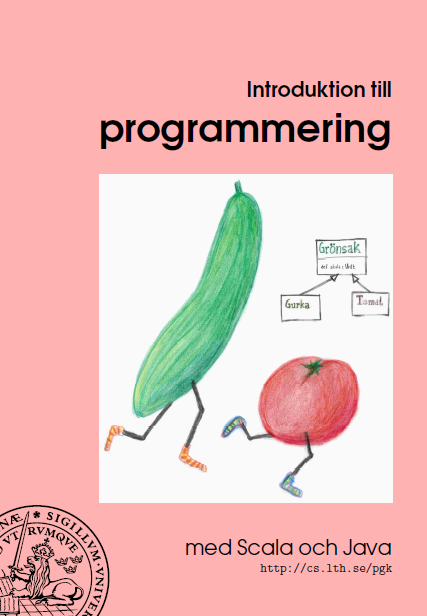
\includegraphics[width=0.65\textwidth]{../img/compendium-front-page.png}
\begin{itemize}
\item \Emph{Kompendium} med övningar \& laborationer, trycks \& säljs av inst. på beställning
\item Föreläsningsbilder
\item Nätresurser enl. länkar

\end{itemize}
\end{minipage}
\hskip1em\begin{minipage}{0.5\textwidth}\SlideFontSize{8}{10}
Bra, men ej nödvändig, \Emph{bredvidläsning}:\\ 
-- för \Emph{nybörjare}:
\vskip0.2mm

\includegraphics[width=0.33\textwidth]{../img/lewisbook.jpg}\hskip4mm

\includegraphics[width=0.33\textwidth]{../img/ankbok.jpg}

\noindent -- för de som \Emph{redan kodat} en del:
\vskip0.7mm
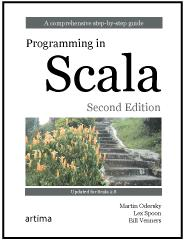
\includegraphics[width=0.45\textwidth]{../img/pinsbook.jpg}\hskip4mm

\includegraphics[width=0.47\textwidth]{../img/koffmanbook.jpg}
\end{minipage}
\end{Slide}

\ifkompendium
\noindent Kompendiet är den huvudsakliga kurslitteraturen och definierar kursinnehållet. Föreläsningar, övningar och laborationer i kompendiet är kursens primära kunskapskällor, tillsammans med de öppna resurser på nätet som kompendiet hänvisar till. Kompendiet är öppen källkod och du välkomnas varmt att bidra!

Om du gärna vill ha en eller flera mer traditionella läroböcker som bredvidläsning rekommenderas följande:
\begin{itemize}[noitemsep, leftmargin=*]
\item För de som aldrig kodat, och vill läsa om kodning från grunden:
\begin{itemize}[nolistsep]
\item ''Introduction to Programming and Problem-Solving Using Scala, Second Edition'', Mark C. Lewis, Lisa Lacher.  {\href{https://www.crcpress.com/Introduction-to-Programming-and-Problem-Solving-Using-Scala-Second-Edition/Lewis-Lacher/p/book/9781498730952}{www.crcpress.com/Introduction-to-Programming-and-Problem-Solving-Using-Scala-Second-Edition/Lewis-Lacher/p/book/9781498730952}}
\item ''Objektorienterad programmering och Java'', Per Holm, Tredje upplagan (2007). \href{https://www.studentlitteratur.se/#6735}{www.studentlitteratur.se/\#6735}
\end{itemize}
\item För de som redan kodat en hel del i ett objektorienterat språk:
\begin{itemize}[nolistsep, noitemsep]
\item ''Programming in Scala, Third Edition -- A comprehensive step-by-step guide'', Martin Odersky, Lex Spoon, and Bill Venners. \\ \href{http://www.artima.com/shop/programming_in_scala_3ed}{www.artima.com/shop/programming\_in\_scala\_3ed} 
\item ''Data Structures: Abstraction and Design Using Java, 3rd Edition'', Elliot B. Koffman, Paul A. T. Wolfgang. \\
\href{http://eu.wiley.com/WileyCDA/WileyTitle/productCd-1119186528.html}{http://eu.wiley.com/WileyCDA/WileyTitle/productCd-1119186528.html}
\end{itemize}
\end{itemize}
Dessa läroböcker följer inte direkt kursens upplägg vad gäller omfång och progression och du får själv göra den nyttiga hemläxan att koppla  deras innehåll till det vi går igenom i kursens olika moduler.

\else
\begin{Slide}{Beställning av kompendium och snabbreferens}\SlideFontSmall
\begin{itemize}
\item \Emph{Kompendiet} finns i pdf för fri nedladdning enl. CC-BY-SA, men det \Alert{rekommenderas starkt} att du köper den tryckta bokversionen.
\item Det är mycket lättare att ha övningar och labbar \Alert{på papper} \Emph{bredvid skärmen}, när du ska tänka, koda och plugga!
\item \Emph{Snabbreferensen} finns också i pdf men du behöver ha en tryckt version eftersom det är \Alert{enda tillåtna hjälpmedlet} på skriftliga kontrollskrivningen och tentamen.
\item Kompendiet och snabbreferens trycks här i E-huset och säljs av institutionen till självkostnadspris. Pris för kompendium+snabbreferens \Alert{beror på hur många som beställer}.
\item Snabbreferens enbart kostar 10 kr.
\item Skriv upp dig på listan -- tryckning sker efter beställning.
\item Du betalar \Alert{kontant} med \Emph{jämna pengar} på cs expedition, våning 2.
\end{itemize}
\end{Slide}
\fi

\ifkompendium\else
\begin{Slide}{Personal}\SlideFontSmall
\begin{description}
\item [\bfseries Kursansvarig:] ~\\Björn Regnell, bjorn.regnell@cs.lth.se
\item [\bfseries Kurssekreterare:]  ~\\Lena Ohlsson \\Exp.tid 09.30 -- 11.30 samt 12.45 -- 13.30
\item [\bfseries Handledare:] ~\\
\Emph{Doktorander}: \\ 
Tekn. Lic. Maj Stenmark, Gustav Cedersjö\\
\Emph{Teknologer}: \\
Anders Buhl, 
Anna Palmqvist Sjövall, 
Anton Andersson,
Cecilia Lindskog, 
Emil Wihlander, 
Erik Bjäreholt, 
Erik Grampp, 
Filip Stjernström, 
Fredrik Danebjer, 
Henrik Olsson, 
Jakob Hök, 
Jonas Danebjer, 
Måns Magnusson, 
Oscar Sigurdsson, 
Oskar Berg, 
Oskar Widmark, 
Sebastian Hegardt, 
Stefan Jonsson, 
Tom Postema, 
Valthor Halldorsson
\end{description}
\end{Slide}
\fi

\begin{Slide}{Föreläsningsanteckningar}
\begin{itemize}
\item Föreläsningsanteckningar utvecklas under kursens gång
\item Några av bilderna finns i kompendiet
\item Alla bilder läggs ut här: \\
\href{https://github.com/lunduniversity/introprog/tree/master/slides}{github.com/lunduniversity/introprog/tree/master/slides} \\
och uppdateras kontinuerligt allt eftersom de utvecklas
\item Förslag på förbättringar välkomna!
\end{itemize}
\end{Slide}

\begin{Slide}{Kursmoment --- varför?}\SlideOnly{\footnotesize}
\begin{itemize}
\item \Emph{Föreläsningar}: skapa översikt, ge struktur, förklara teori, svara på frågor, motivera varför
\item \Emph{Övningar}: \Alert{förbereda} laborationerna, bearbeta teorins olika delar med avgränsade deluppgifter, \Emph{grundövningar} för alla, \Emph{extraövningar} om du vill/behöver öva mer, \Emph{fördjupningsövningar} om du vill gå djupare 
\item \Emph{Laborationer}: \Alert{obligatoriska}, sätta samman teorins delar i ett större program; lösningar redovisas för handledare; gk på alla för att få tenta, 
\item \Emph{Resurstider}: få hjälp med övningar och laborationsförberedelser av handledare, fråga vad du vill
\item \Emph{Samarbetsgrupper}: grupplärande genom samarbete, hjälpa varandra 
\item \Emph{Kontrollskrivning}: \Alert{obligatorisk}, diagnostisk, kamraträttad; kan ge samarbetsbonuspoäng till tentan
\item \Emph{Individuell projektuppgift}: \Alert{obligatorisk}, du visar att du kan skapa ett större program självständigt; redovisas för handledare
\item \Emph{Tentamen}: \Alert{obligatorisk}, skriftlig, enda hjälpmedel: snabbreferensen\\   \url{http://cs.lth.se/pgk/quickref}
\end{itemize}
\end{Slide}

\ifkompendium\else
\begin{Slide}{Detta är bara början... }
Exempel på efterföljande kurser som bygger vidare på denna:
\begin{itemize}
\item Årskurs 1
\begin{itemize}
\item Programmeringsteknik -- fördjupningskurs
\item Utvärdering av programvarusystem
\item Diskreta strukturer
\end{itemize}
\item Årskurs 2
\begin{itemize}
\item Objektorienterad modellering och design
\item Programvaruutveckling i grupp
\item Algoritmer, datastrukturer och komplexitet
\item Funktionsprogrammering
\end{itemize}
\end{itemize}
\end{Slide}


\begin{Slide}{Registrering}
\begin{itemize}
\item Fyll i listan som skickas runt.
\item Kryssa i kolumnen \Emph{Ska gå} om du ska gå kursen\footnote{\scriptsize D1:a som redan gått motsvarande högskolekurs? Uppsök studievägledningen}\footnote{\scriptsize D2:a eller äldre som vill bli omregistrerad? Prata med kursansvarig på rasten}
\item Kryssa i kolumnen \Emph{Kursombud} om du kan tänka dig att vara kursombud under kursens gång
\begin{itemize}
\item Alla LTH-kurser ska utvärderas under kursens gång och efter kursens slut.
\item Till det behövs kursombud -- ungefär 2 D-are och 2 W-are.
\item Ni kommer att bli kontaktade av studierådet. \\SRD ordf: Amelia Andersson
\end{itemize}
\end{itemize}
\end{Slide}

%%%
\begin{Slide}{Förkunskaper}
\begin{itemize}
\item Förkunskaper $\neq$ Förmåga
\item Varken kompetens eller personliga egenskaper är statiska 
\item ''Programmeringskompetens'' är inte \textit{en} enda enkel förmåga utan en komplex sammansättning av flera olika förmågor som utvecklas genom hela livet
\item Ett innovativt utvecklar\Alert{team} behöver många olika kompetenser för att vara framgångsrikt
\end{itemize}
\end{Slide}

%%%
\begin{Slide}{Förkunskapsenkät}
\begin{itemize}
\item Om du inte redan gjort det fyll i förkunskapsenkäten \Alert{snarast}:
\url{http://cs.lth.se/pgk/survey} 
\item Dina svar behandlas internt och all redovisad statistik anonymiseras.
\item Enkäten ligger till grund för randomiserad gruppindelning i samarbetsgrupper, så att det blir en spridning av förkunskaper inom gruppen.
\item Gruppindelnig publiceras här: \\ \url{http://cs.lth.se/pgk/grupper/}
\end{itemize}
\end{Slide}

\begin{Slide}{Samarbetgrupper}\footnotesize
\begin{itemize}
\item Ni delas in i \Emph{samarbetsgrupper} om ca 5 personer baserat på förkunskapsenkäten, så att olika förkunskapsnivåer sammanförs
\item Några av laborationerna är mer omfattande \Emph{grupplabbar} och kommer att göras i samarbetsgrupperna \\ \vspace{1em}
\item Kontrollskrivningen i halvtid kan ge \Emph{samarbetsbonus} (max 5p) som adderas till ordinarie tentans poäng (max 100p) med medelvärdet av gruppmedlemmarnas individuella kontrollskrivningspoäng 
\scriptsize \parbox{7cm}{Bonus $b$ för varje person i en grupp med $n$ medlemmar med $p_i$ poäng vardera på kontrollskrivningen:} 
 \hspace{5mm} $\displaystyle b = \sum\limits_{i=1}^n \frac{p_i}{n}$
\end{itemize}
\end{Slide}

\fi

%%%
\begin{Slide}{Varför studera i samarbetsgrupper?}

Huvudsyfte: \Emph{Bra lärande!}

\begin{itemize}
\item Pedagogisk forskning stödjer tesen att lärandet blir mer djupinriktat om det sker i utbyte med andra
\item Ett studiesammanhang med höga ambitioner och respektfull gemenskap gör att vi \Emph{når mycket längre}
\item Varför ska du som redan kan mycket aktivt dela med dig av dina kunskaper?
\begin{itemize}
\item Förstå bättre själv genom att förklara för andra
\item Träna din pedagogiska förmåga
\item Förbered dig för ditt kommande yrkesliv som mjukvaruutvecklare 
\end{itemize}
\end{itemize}
\end{Slide}

%%%

\ifkompendium\else
\begin{Slide}{Samarbetskontrakt}
Gör ett skriftligt \href{https://github.com/bjornregnell/lth-eda016-2015/blob/master/assignments/collaboration-contract.tex}{\bf samarbetskontrakt} med dessa och ev. andra punkter som ni också tycker bör ingå:
\begin{enumerate}
\item Återkommande mötestider per vecka
\item Kom i tid till gruppmöten
\item Var väl förberedd genom självstudier inför gruppmöten
\item Hjälp varandra att förstå, men ta inte över och lös allt
\item Ha ett respektfullt bemötande även om ni har olika åsikter
\item Inkludera alla i gemenskapen
\end{enumerate}

Diskutera hur ni ska uppfylla dessa innan alla skriver på. \\ Ta med samarbetskontraktet och visa för handledare på labb 1.

\vskip1em

\Alert{Om arbetet i samarbetsgruppen inte fungerar ska ni mejla kursansvarig och boka mötestid!}
\end{Slide}

\begin{Slide}{Bestraffa inte frågor!}
\begin{itemize}
\item Det finns bättre och sämre frågor vad gäller hur mycket man kan lära sig av svaret, men \Emph{all undran är en chans} att i dialog utbyta erfarenheter och lärande
\item Den som frågar \Emph{vill veta} och berättar genom frågan något om nuvarande kunskapsläge
\item Den som svarar får chansen att \Emph{reflektera} över vad som kan vara svårt och olika vägar till djupare förståelse
\item I en hälsosam lärandemiljö är det \Emph{helt tryggt} att visa att man ännu inte förstår, att man gjort ''fel'', att man har mer att lära, etc. 
\item Det är viktigt att våga försöka även om det blir ''fel'':\\ \Emph{det är ju då man lär sig!}
\end{itemize}
\end{Slide}

%%%
\begin{Slide}{Plagiatregler}
Läs dessa regler noga och diskutera i samarbetsgrupperna:
\begin{itemize}
\footnotesize
\item \url{http://cs.lth.se/utbildning/samarbete-eller-fusk/}
\item \url{http://cs.lth.se/utbildning/foereskrifter-angaaende-obligatoriska-moment/}
\end{itemize}
Ni ska lära er genom \Emph{eget arbete} och genom  \Emph{bra samarbete}. Samarbete gör att man lär sig bättre, men man lär sig inte av att bara kopiera andras lösningar. Plagiering är förbjuden och kan medföra disciplinärende och avstängning.
\end{Slide}

\fi %%%%%%%%%%%%%%%%%%%%%%%%%%%%%%%%

%%%
\begin{Slide}{En typisk kursvecka}
\begin{enumerate}
\item Gå på \Emph{föreläsningar} på \Alert{måndag--tisdag}
\item Jobba med \Emph{individuellt} med teori, övningar, labbförberedelser på  \Alert{måndag--torsdag}
\item Kom till \Emph{resurstiderna} och få hjälp och tips av handledare och kurskamrater på \Alert{onsdag--torsdag}
\item Genomför den obligatoriska \Emph{laborationen} på \Alert{fredag}
\item Träffas i \Emph{samarbetsgruppen} och hjälp varandra att förstå mer och fördjupa lärandet, förslagsvis på återkommande tider varje vecka då alla i gruppen kan
\end{enumerate}
Se detaljerna och undantagen i schemat: \href{http://cs.lth.se/pgk/schema}{cs.lth.se/pgk/schema}
\end{Slide}

\ifkompendium\else  %%%%%%%%%%%%%%%%%%%%%%%%%
%%%
\begin{Slide}{Laborationer}\footnotesize
\begin{itemize}
\item \Alert{Programmering lär man sig bäst genom att programmera...}
\item Labbarna är \Emph{individuella} (utom 2) och \Emph{obligatoriska}
\item Gör övningarna och labbförberedelserna noga \textit{innan} själva labben -- detta är ofta helt nödvändigt för att du ska hinna klart. Dina labbförberedelserna kontrolleras av handledare under labben.
\item Är du sjuk? Anmäl det \Alert{före} labben till \url{bjorn.regnell@cs.lth.se}, \\ få hjälp på resurstid och redovisa på resurstid (eller labbtid, när handledaren har tid över)
\item Hinner du inte med hela? Se till att handledaren noterar din närvaro, och fortsätt på resurstid och ev. uppsamlingstider.
\item Läs noga anvisningarna i kompendiet
\item Laborationstiderna är gruppindelade enligt \href{http://cs.lth.se/eda016/schema/}{schemat}. Du ska gå till den tid och den sal som motsvarar din \href{http://cs.lth.se/eda016/grupper/}{grupp}.
\end{itemize}
\end{Slide}

%%%
\begin{Slide}{Resurstider}
\begin{itemize}
\item På resurstiderna får du hjälp med övningar och laborationsförberedelser
\item Kom till minst en resurstid per vecka (se \href{http://cs.lth.se/eda016/schema/}{schema})
\item Handledare gör ibland \Emph{genomgångar} för alla under resurstiderna. Tipsa om handledare om vad du finner svårt.
\item Resurstiderna är inte gruppindelade i schemat. Du får i mån av plats gå på flera resurstider per vecka. Om det blir fullt i ett rum prioriteras dessa grupper för att minimera schemakrockar: 
\end{itemize}
\begin{table}[]
\centering\scriptsize
\begin{tabular}{lllll}
Tid Lp1 & Sal & Grupper med prio \\
\hline
Ons 10-12 v1-7 & Hacke  &   09 \& 10 \\
Ons 13-15 v1-7 & Hacke  &   07 \& 08  \\
Ons 15-17 v1-7 & Panter  & 05 \& 06   \\
Ons 15-17 v1-7 & Val       &  03 \& 04   \\
Tor 13-15 v1-7 & Mars     & 01 \& 02  \\
Tor 15-17 v1-7 & Mars     & 11 \& 12 \\ 
\end{tabular}
\end{table}
\end{Slide}

\fi
%!TEX root = ../lect-week01.tex

%%%%%%%%%%%%%%%%%%%%%%%%%%%%%%%%%%%%%%
\Subsection{Om programmering}

%%%

\begin{Slide}{Att skapa koden som styr världen}
\begin{multicols}{2}\footnotesize
I stort sett alla delar av samhället är beroende av programkod:
\begin{itemize}\scriptsize
\item kommunikation
\item transport
\item byggsektorn
\item statsförvaltning
\item finanssektorn
\item media \& underhållning
\item sjukvård
\item övervakning
\item integritet
\item upphovsrätt
\item miljö \& energi
\item sociala relationer
\item utbildning 
\item ...
\end{itemize}
\columnbreak %---------
Hur blir ditt framtida yrkesliv som systemutvecklare?
\begin{itemize}
\item  Redan nu är det en skriande brist på utvecklare och bristen blir bara värre och värre... \\
  \href{http://computersweden.idg.se/2.2683/1.634770/rekrytera-utvecklare}{CS 2015-08-17}
\item Störst brist är det på kvinnliga utvecklare: \\
\href{http://www.dn.se/ekonomi/it-branschen-hotas-av-brist-pa-kvinnor/}{DN 2015-04-02}
\item Global kompetensmarknad \\ 
  \href{http://computersweden.idg.se/2.2683/1.630901/det-finns-programmerare-och-sa-finns-det-programmerare}{CS 2015-06-14}\\
   \href{http://computersweden.idg.se/2.2683/1.634700/7-satt-att-bli-en-battre-programmerare}{CS 2015-08-15}
\end{itemize}
\end{multicols}
\end{Slide}


\ifkompendium\noindent
{\scriptsize
\url{http://computersweden.idg.se/2.2683/1.634770/rekrytera-utvecklare}\\
\url{http://www.dn.se/ekonomi/it-branschen-hotas-av-brist-pa-kvinnor}\\
\url{http://computersweden.idg.se/2.2683/1.630901/det-finns-programmerare-och-sa-finns-det-programmerare}
\url{http://computersweden.idg.se/2.2683/1.634700/7-satt-att-bli-en-battre-programmerare}
}
\fi

\begin{Slide}{Utveckling av mjukvara i praktiken}
\begin{itemize}
\item \Emph{Inte bara kodning:} kravbeslut, releaseplanering, design, test, versionshantering, kontinuerlig integration, driftsättning, återkoppling från dagens användare, ekonomi \& investering, gissa om morgondagens användare, ... 
\item \Emph{Teamwork:} Inte ensamma hjältar utan autonoma team i decentraliserade organisationer med innovationsuppdrag
\item \Emph{Snabbhet:} Att koda innebär att hela tiden uppfinna nya ''byggstenar'' som ökar organisationens förmåga att snabbt skapa värde med hjälp av mjukvara. Öppen källkod. Skapa kraftfulla API:er.
\item \Emph{Livslångt lärande:} Lär nytt och dela med dig hela tiden. Exempel på pedagogisk utmaning: hjälp andra förstå och använda ditt API $\implies$ \textit{Samarbetskultur}
\end{itemize}
\end{Slide}

\ifkompendium\else
\SlideImg{Programming unplugged: Två frivilliga?}{../img/unplugged}
\SlideImg{Editera och exekvera ett program}{../img/kojo}
\fi


%%%%%%%%%%%%%%%%%%%%%%%%%%%%%%%%%%%%%%
\ifkompendium\else
\Subsection{Meddelande från \href{http://lth.se/code}{Code@LTH}} 
\fi

\end{document}
